\documentclass[../paper.tex]{subfiles}

\begin{document}

  \subsection{Architecture}

  The goal of this project in terms of the implementation was to
  build a web application that is easily embeddable into a mobile application.
  For this reason we decided on going for a lean front end without too many
  unnecessary dependencies to keep it responsive. Among the key dependencies that
  are necessary is D3.js\footnote{JavaScript visualisation library D3: https://d3js.org}, a JavaScript library for manipulating documents based
  on data. D3 fits the requirements of simple interoperability between
  data and visualisation by manipulating the DOM perfectly.

  Given that the
  visualisation is built around a semantic knowledge graph, a graph database is
  a necessity.

  For the implementation, an instance of  GraphDB\footnote{GraphDB: https://www.ontotext.com/products/graphdb/}, a proprietary graph
  database developed by Ontotext, was used. It offers multiple APIs for querying the database,
  including RDF4J and SPARQL, among other things. The multiple APIs offered by
  GraphDB allowed us to use a vendor-agnostic JavaScript framework for
  creating SPARQL queries. As the overall goal was simplicity and reusability,
  SPARQL was used querying data, since it is widely used
  in the semantic community and well adopted. This makes the application work with
  basically any graph database, which supports data fetching with SPARQL.

  A simple use case would be a user starting the application, which initialises
  the D3 front end web application, which in turn queries data from the database
  to visualise the consent page as shown in \cref{fig:prototype-finish}.
  

  Shown in \cref{fig:architecture} is an overview of the technical architecture
  for the implementation of the data visualisation.

  \begin{figure}
    \centering
    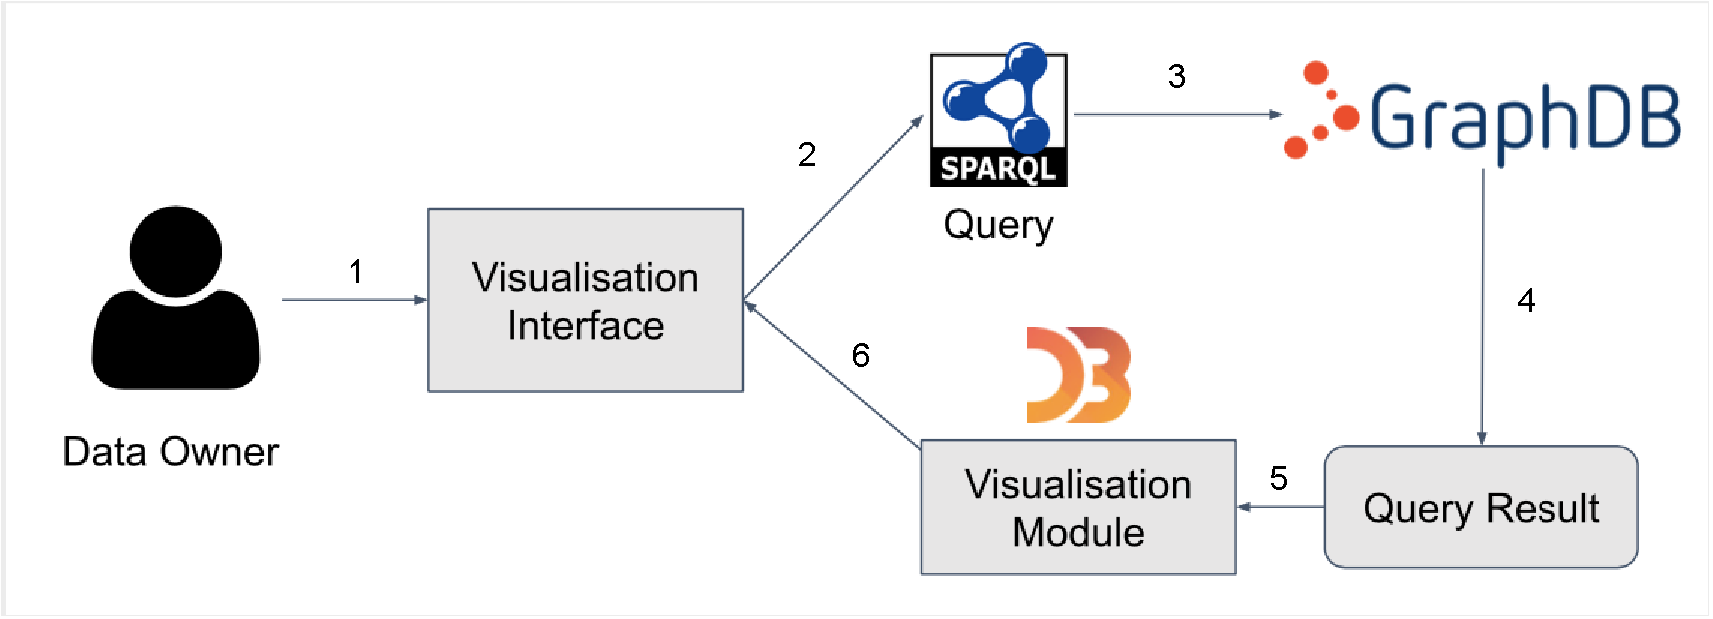
\includegraphics[width=\linewidth]{architecture_numbered.pdf}
    \caption{Technical Architecture}
    \label{fig:architecture}
  \end{figure}

  On the left side of \cref{fig:architecture} we see the application user, i.e.
  the data owner. The data owner interacts only with the front end part of the
  application, which we call the “Visualisation Interface”.

  On first load or whenever the user interacts with the interface in such a way
  that the underlying data needs to be updated, we send a SPARQL query to the
  GraphDB database. Once the result of this query is retrieved, it is passed to
  the “Visualisation Module”. This module processes the data depending on
  whether it will be displayed in the overview visualisation or the detailed
  time series visualisation and produces the corresponding visualisation
  using D3.js accordingly.

  Depending on the query, we get a lot of data in return, as the database
  will return a value for each data-package, that was sent. The so called
  "Visualisation Module" groups those together, creating a single visible
  node for each category of data. These categories are predefined in the
  ontology and represent thing like coordinates, longitude and latitude, or
  fuel consumption. The module then creates connections between the data packages
  and the third party companies receiving them. One can think of this module
  as the pure front end of the application.

  After the visualisation is created for the received data, the “Visualisation Module”
  updates the currently displayed graph. This can easily be done with D3.js, since
  it creates a graph context, which can be modified directly. Therefore,
  we can add or remove nodes from the graph and directly update the visualisation
  upon the receiving a users input.
  
  \subsection{Campaign data}
  Here goes the KG implementation: graphDB + ontology details
  
  \subsection{User interface}
  For the first prototype of our application the idea was to learn from
  previously done work and reuse what worked best. Additionally we followed
  general design principles like Gestalt laws \cite{wiki:principles_of_grouping}
  of grouping.

  A typical visualisation technique to make complex relationships clearly
  understandable is a graph layout. To show data flow from a data subject to one
  or more data processors, a graph works very well. Nodes represent data
  subject and data processors, and the links between them show that they relate
  with each other in such a way that data is shared between them. To make this
  even more clear, actual or imaginary data packets can be visualised as moving
  particles between the nodes. This feature makes it possible to give the
  visualisation a sense of directional flow.
  These design choices are also backed by Gestalt laws such as the law of
  similarity, which states that visual objects resembling each other are
  perceived as belonging to the same group. Further, the law of common fate
  states that objects moving into the same direction are recognised as grouped
  such as the data stream in the visualisation.

  \begin{figure}[H]
    \centering
    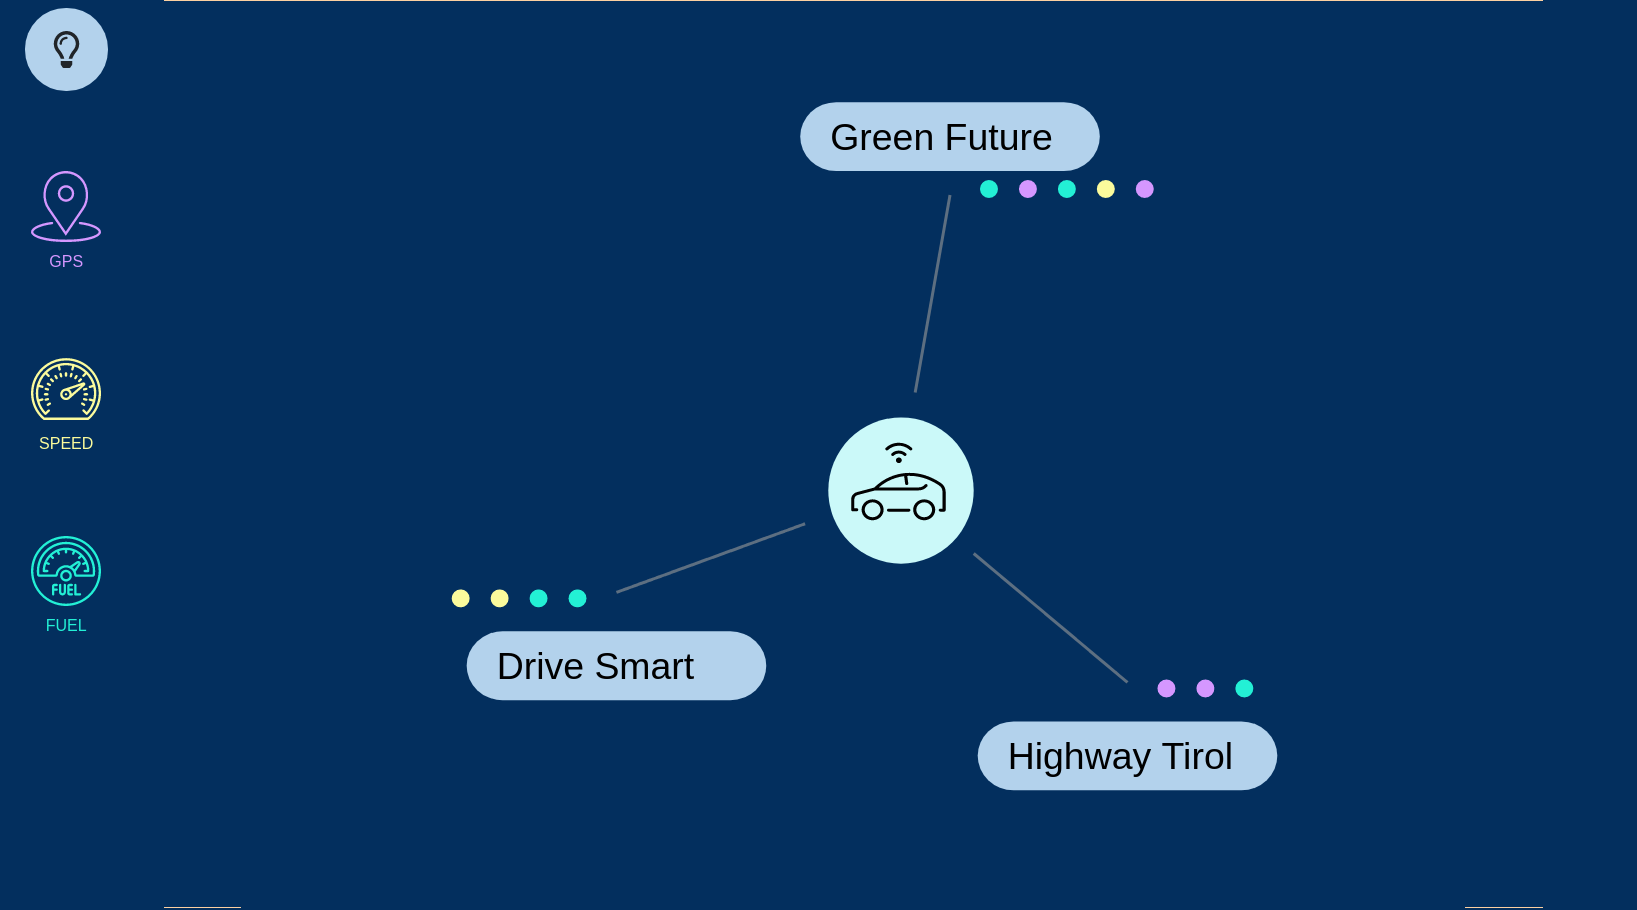
\includegraphics[width=\linewidth]{prototype-finish}
    \caption{The finished prototype of the general view}
    \label{fig:prototype-finish}
  \end{figure}

  Since the whole application is built around giving users a sense of control
  over their sharing activities, the user as a data subject stands in the centre of
  the visualisation with the connected data processors distributed around in a
  circle with the centre point
  being the user. Data processors, called campaigns in the CampaNeo environment, are
  represented by a rounded rectangle and the corresponding campaign name. The round
  particles represent data packets flowing from the user to the campaign. They are
  colour-coded to give additional information on the type of data that is sent,
  e.g. fuel consumption, speed or the GPS location of the car.
  The meaning of the different colours are encoded in a legend on the bottom left
  side of the screen. Here, words are paired with unambiguous symbols to make the
  legend easier and faster to read and understand. On the whole, the visualisation
  is designed to enable users to see at one glance what kind of data they are sharing
  and at what rate indicated by the data particle animation.

  With that we have now completely satisfied the defined needs of our application:
  The user can now find out with whom he shares what data and approximately at what
  rate. However, in case the user wants to get more in-depth information, it is
  possible to click on a specific data flow in the visualisation in order
  to get a more detailed view of the data stream. Here we rely on a time series
  visualisation and give additional information about the sensor that retrieved
  the data and the companies, with whom the data processor shares the collected data.
  
\begin{figure}[H]
    \centering
    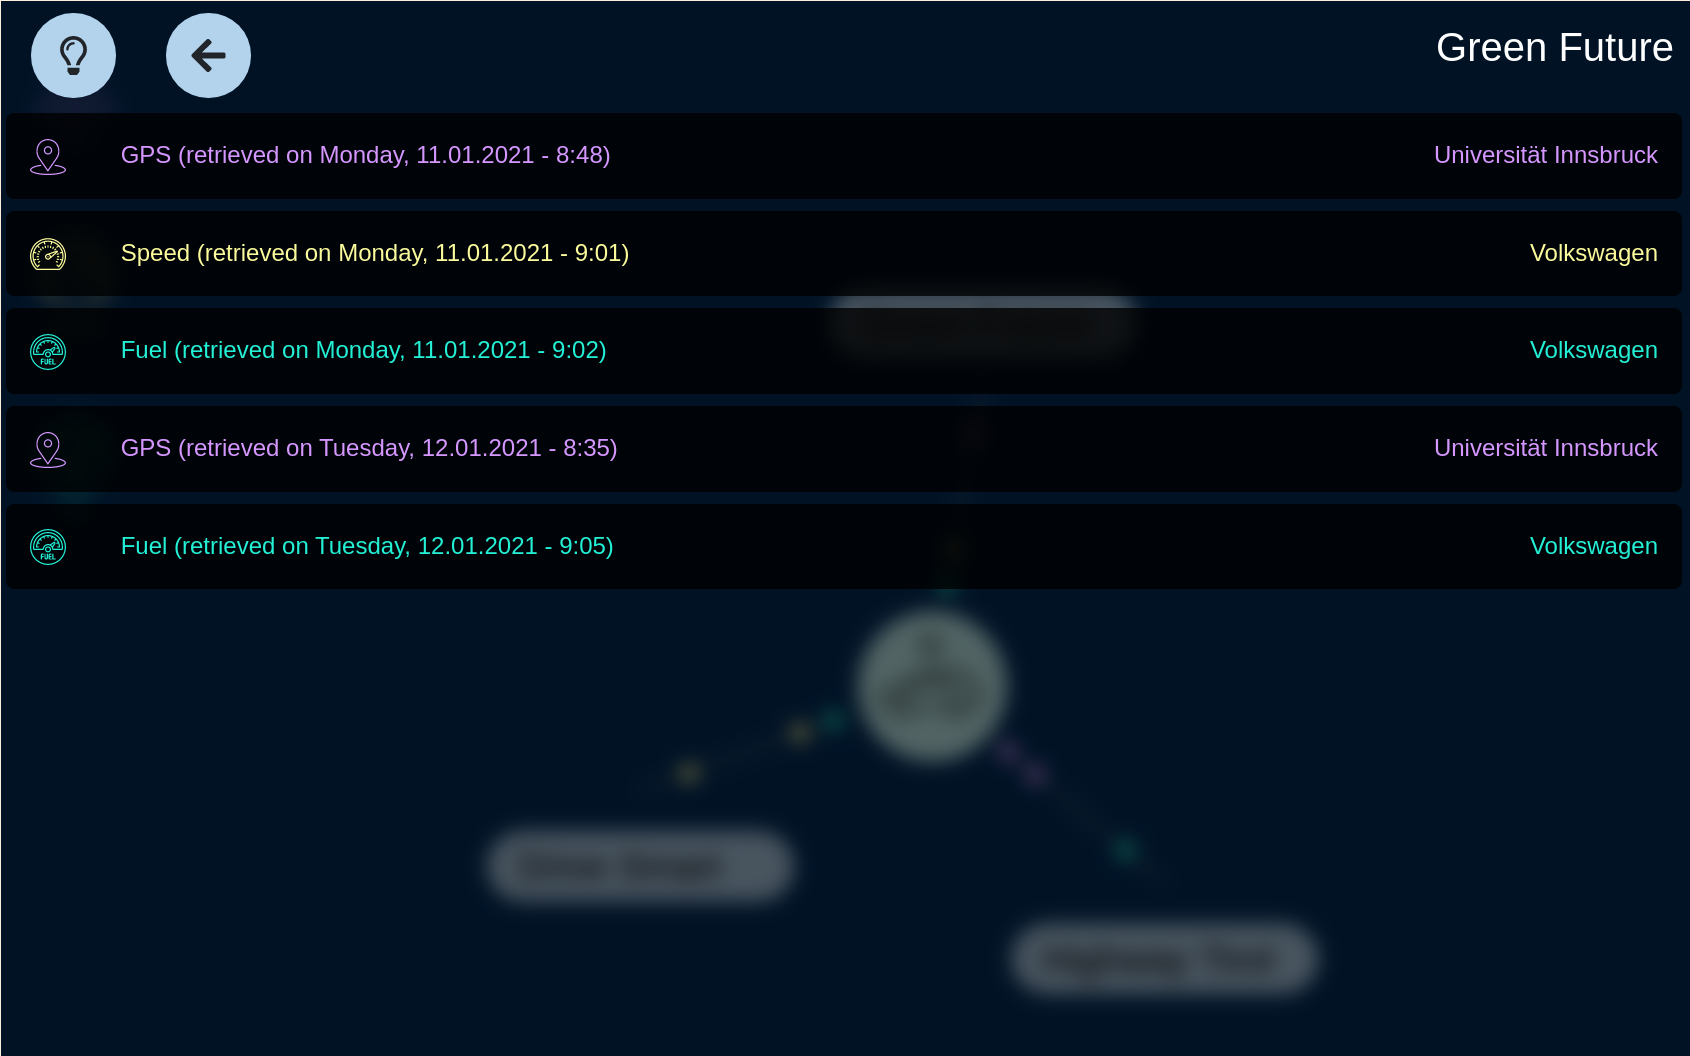
\includegraphics[width=\linewidth]{prototype-detail}
    \caption{Detailed view of campaign data}
    \label{fig:prototype-detail}
  \end{figure}
%
%  \begin{figure}[H]
%    \centering
%    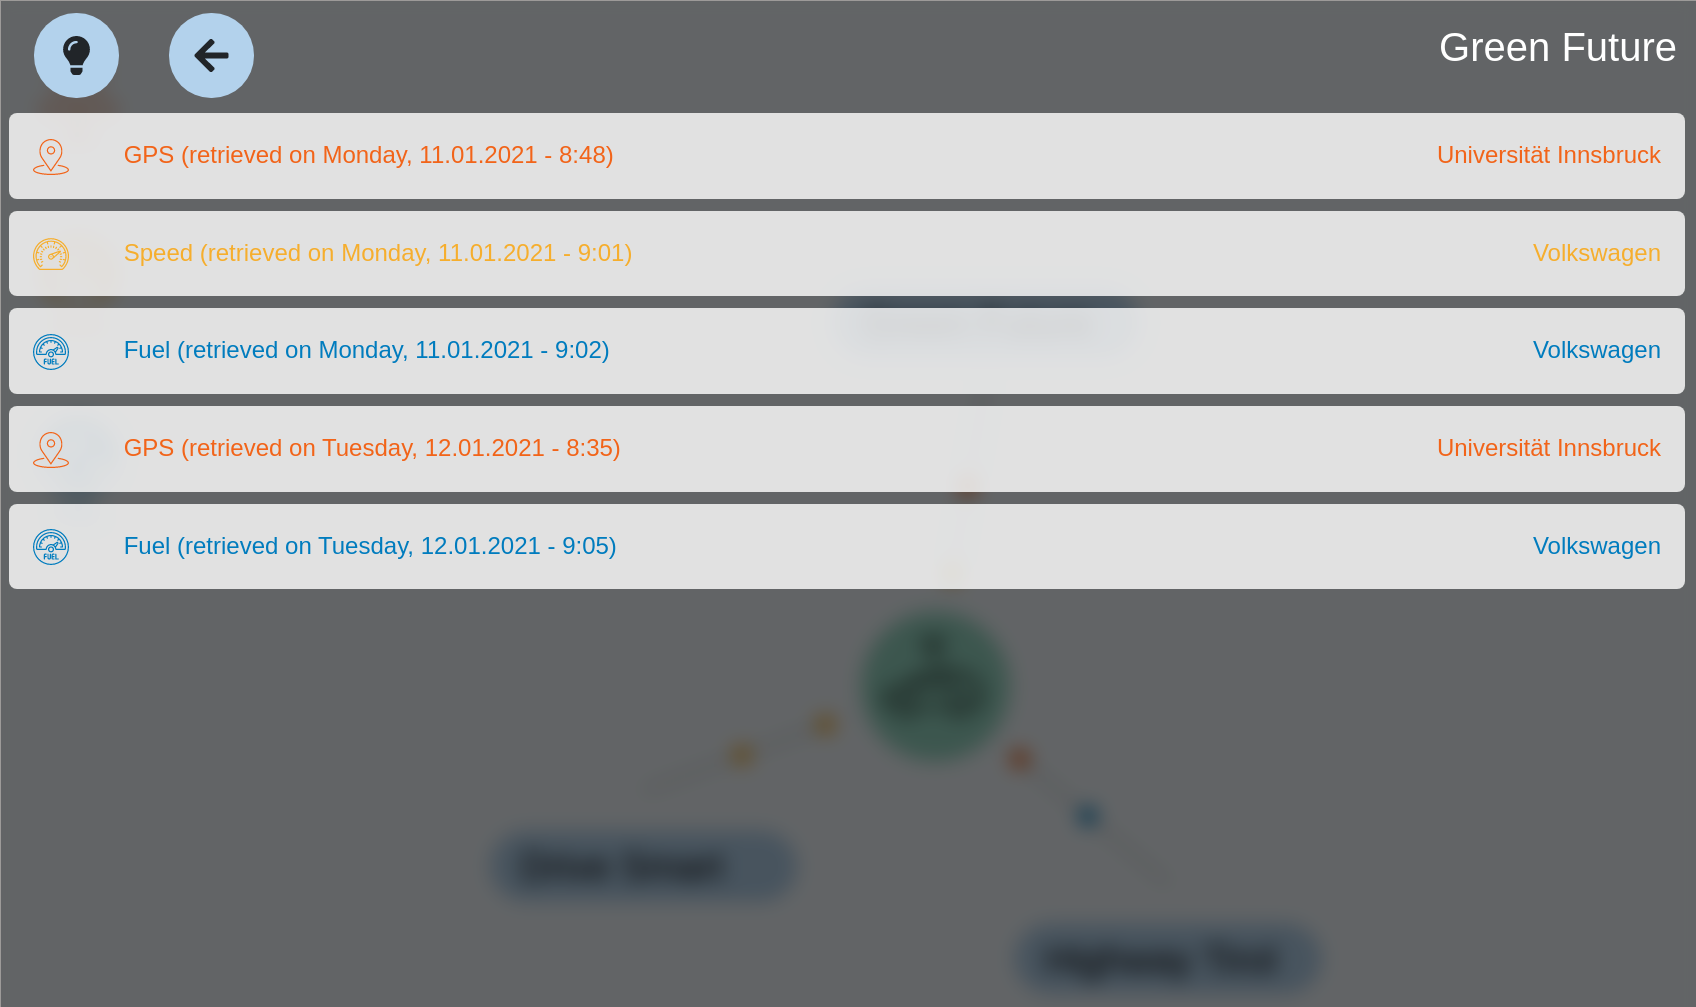
\includegraphics[width=\linewidth]{prototype-detail-light}
%    \caption{Detailed view of a campaign with light colour scheme}
%    \label{fig:prototype-detail-light}
%  \end{figure}
% 
  Clarity is of utmost importance, which is why the visualisation always starts
  with the summary view to avoid confusing the user with too much information
  at once. The more detailed information is served only upon interacting with
  the visualisation. Displaying everything on screen at the same time would
  overload the initial rendering far too much. The moving particles, representing the
  data packets, are designed to directly draw a users attention on the centre of the
  application. Therefore, the animation of the flow is implemented as a loop, i.e.
  after the particles have arrived at their destination, they stay there for a short
  time before disappearing and flowing again from the centre.

  The finished prototype has gone through quite some iterations, to improve
  the usability as well as design in general. Among the main changes from the
  initial prototype is the ability to scale the graph according to the device, which
  makes the UI usable across many devices. The position of the legend has changed
  as well to make it more uniform as a side bar with the newly added ``light switch''
  button, which as the name suggests adds the ability to change the colours of
  the whole user interface. The detailed view itself offers detailed information
  of the shared data as well as to whom the consent has been given. Furthermore
  an easily accessible ``back'' button has been added, which leads the user back
  to the general view.

\end{document}
